\chapter{Binomial Array}	
In the previous section, we discussed the Schelkuhoff method where we investigated arrays whose radiation pattern specified in terms of its nulls. We saw that if the radiation pattern is specified in terms of the nulls, then we can synthesize an array by using circle diagram. However in this section we discuss the binomial array which decouples the relationship between directivity and number of nulls of an antenna array. As we have seen the number of elements in an array increases the number of nulls and also increases the directivity (because as the size of an array increases, the beam width decreases). The analytical formulation of the technique is as follows

Let's consider a 2 element array and specify the radiation pattern from the schelkunoff therom as follows.\\
\begin{figure}[h]
\centering
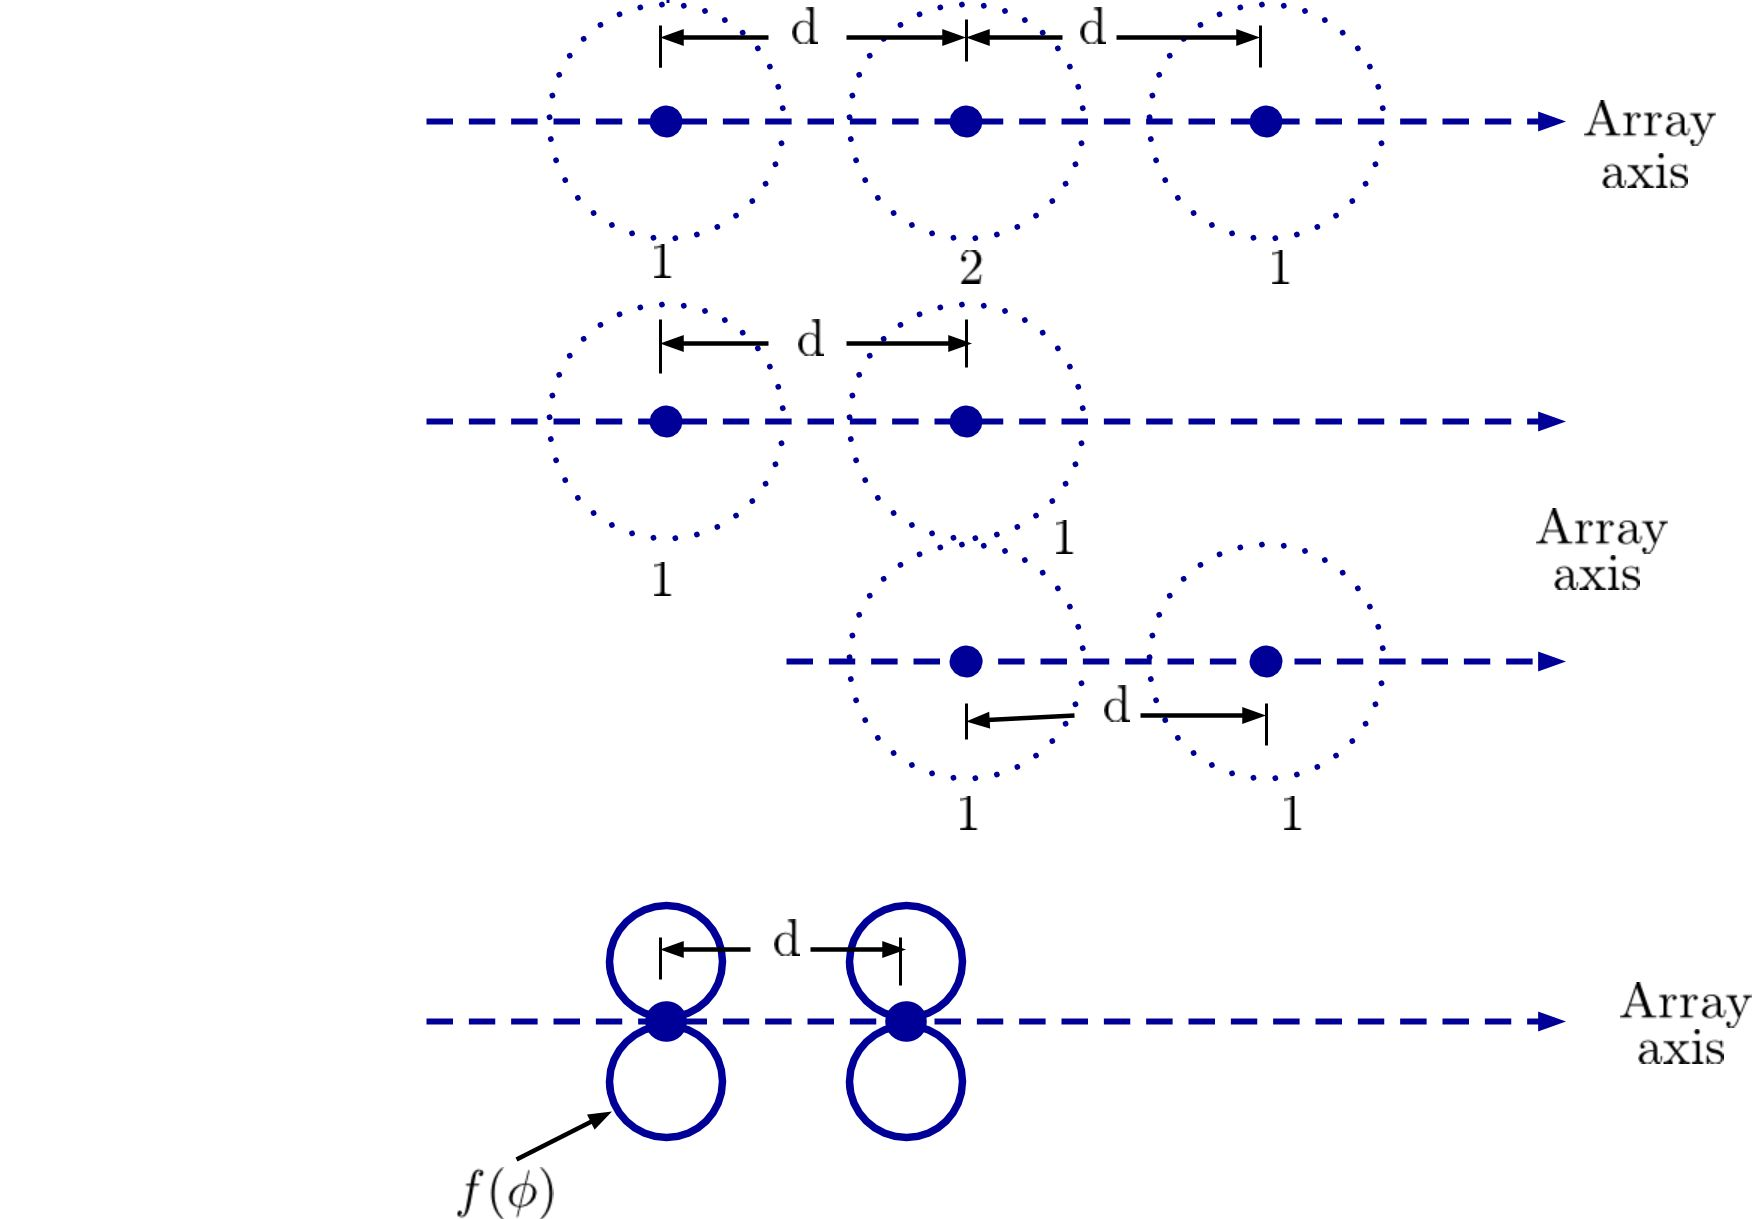
\includegraphics[width=1\linewidth]{/graphics/img59_9}
\caption{}
\label{fig:fig-11}
\end{figure}

The radiation pattern $AF = |1 + e^{j\psi}| = |1 + z| \; \; \; \; \; \text{where} \; \; z =  e^{j\psi}$. For this array we have a null when $z = -1 =  e^{j\psi}$. To increase the directivity and not affect the number of nulls we increase the number of element to a (N + 1) element array such that the array factor is a Nth power polynomial of (1 + z) so that the null is at $\zeta = -1$. So now there is freedom to control the directivity.\\
Therefore, $AF = |(1 + z)^N|$ and the Binomial expression gives 
\begin{equation}
AF = 1\;  +\;  {^NC_1z} \; +\; \; {^NC_2z^2} +\; \; {^NC_3z^3} \; + \ldots
\label{eqn51}
\end{equation}
Where the coefficient of the polynomial corresponds to the excitation of the antenna array. Equation~\ref{eqn51} can be rewritten as;
\begin{equation}
1 + Nz + \dfrac{N(N - 1)}{2!}\cdot z^2 + \dfrac{N(N - 1)(N - 2)}{3!}\cdot z^3 + \ldots\label{eqn52}
\end{equation}
The positive coefficient of the series expansion for different values of N are:\\

N = 0\; \; \; \; \; \; \; \; \; \; \; \; \; \; \;\; \; \; \; \; 1\\

N = 1\; \; \; \; \; \; \; \; \; \; \; \; \; \; \;\; \; \; 1 \; \; \; 1\\

N = 2\; \; \; \; \; \; \; \; \; \; \; \; \; \; \;\; 1 \; \; \; 2 \; \; \; 1\\

N = 3\; \; \; \; \; \; \; \; \; \; \; \; \; \;1 \; \; \; 3 \; \; \; 3 \; \; \; 1\\

N = 4\; \; \; \; \; \; \; \; \; \; \; \;1 \; \; \; 4 \; \; \; 6 \; \; \; 4 \; \; \; 1 \\

N = 5\; \; \; \; \; \; \; \; \; \;1 \; \; \; 5 \; \; \;10 \; \; \;10 \; \; \;5 \; \; \; 1\\

N = 6\; \; \; \; \; \; \; \;1 \; \; \; 6 \; \; \;15 \; \; \;20 \; \; \;15 \; \; \;6 \; \; \;1\\

N = 7\; \; \; \; \; \;1 \; \; \; 7 \; \; \;21 \; \; \;35 \; \; \;35 \; \; \;21 \; \; \;7 \; \; \;1\\

N = 8\; \; \; \;1 \; \; \; 8 \; \; \;28 \; \; \;56 \; \; \;70 \; \; \;56 \; \; \;28 \; \; \;8 \; \; \;1\\

N = 9\; \; \;1  \; \; 9 \; \; \;36 \; \; \;84 \; \;\;126\; \; 126\; \; \;84 \; \; \;36 \; \; \;9 \; \; \;1\\

\begin{figure}[h]
\centering
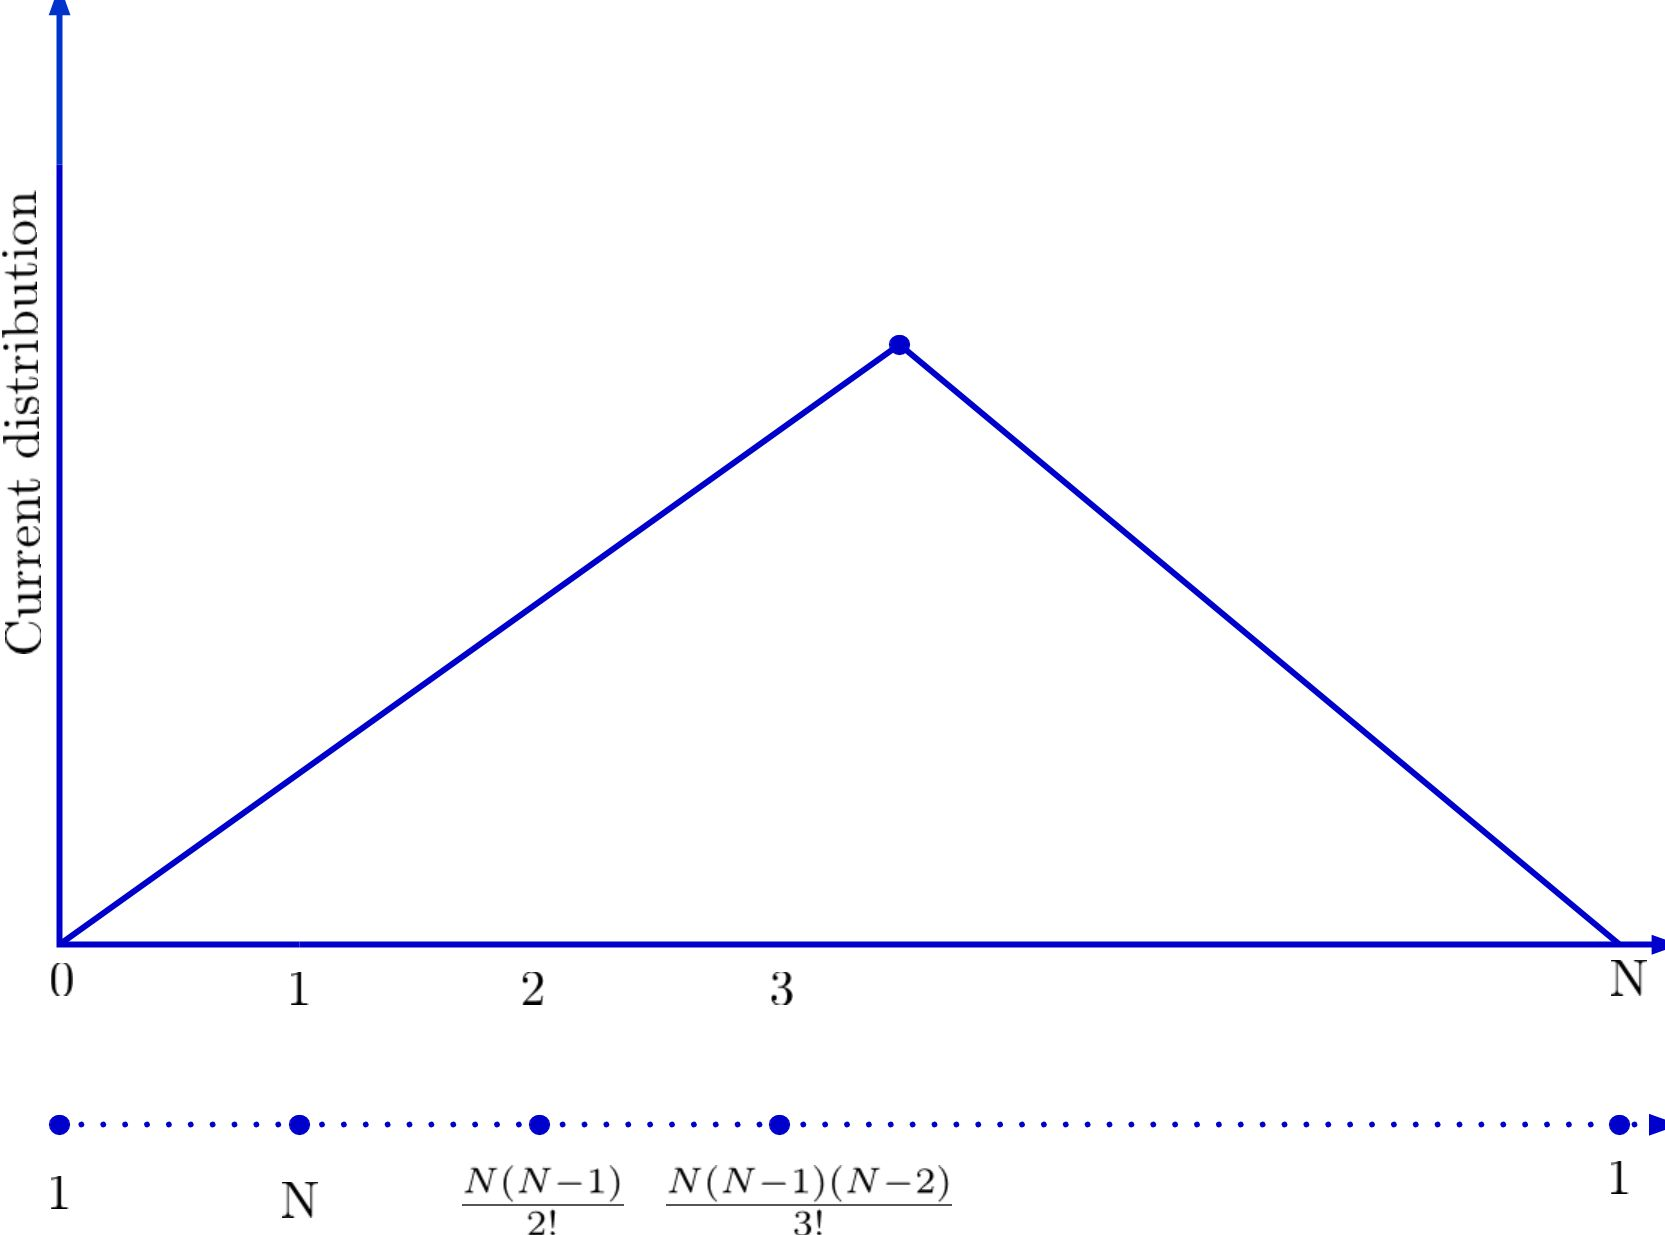
\includegraphics[width=1\linewidth]{graphics/img59_2}
\caption{Current distribution for null}
\label{fig:fig-1}
\end{figure}
The above represents Pascal's triangle\footnote{\textcolor{red}{Blaise Pascal was a French mathematician, physicist, inventor, writer and Catholic theologian In mathematics, Pascal's triangle is a triangular array of the binomial coefficients.}}. Since the coefficients are determined from a binomial series expansion, the array is know as a binomial array. One of the figure of merits of this array is the minimum side lobe level due to the current distribution, also the binomial arrays do not exhibit any minor lobes provided the spacing between the elements is equal or less than $\dfrac{\lambda}{2}$.\\

\section{Design Procedures.}
Let consider a 3 element array $(N + 1 = 3)$, therefore, the binomial array will correspond to any array factor , AF of $(1 + z)^2$.\\
When we consider any array we assume the individual element has radiation pattern which is isotropic in all directions. However, to better analyze this problem, we would consider an antenna array of N elements whose primary radiation pattern is not isotropic, i.e it has a radiation pattern given as $f(\theta,\phi)$ as shown in fig.56-2.

\begin{figure}[h]
\centering
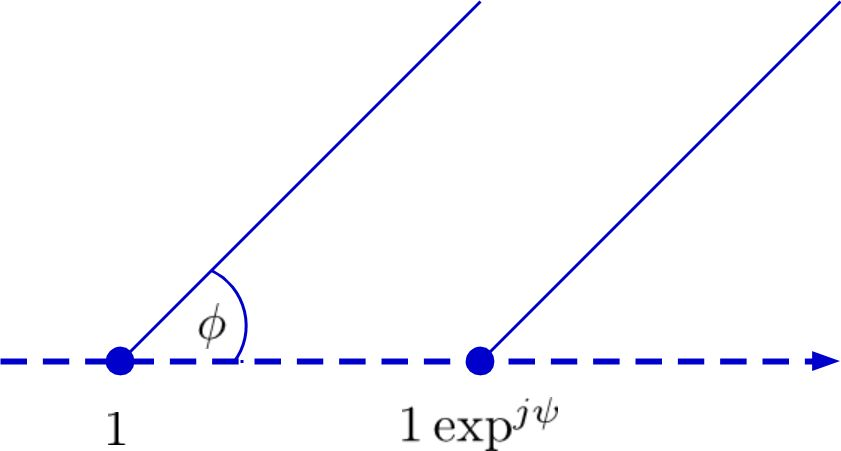
\includegraphics[width=1\linewidth]{/graphics/img59_1}
\caption{N element array of primary radiation pattern $f(\theta, \phi)$}
\label{fig:fig-2}
\end{figure}
If we consider a direction $\phi$ with respect to the array axis, we will observe now that the radiation pattern is affected by the array configuration and the primary array pattern of each antenna element. Lets write the radiation pattern first while ignoring the individual radiation pattern which is given as: 
$$I_1 e^{j0} + I_2 e^{j\psi} + I_3 e^{j2\psi} + \cdots + I_N e^{jN\psi}$$
where $\psi = \beta d\cos\phi + \delta$ and $I_0, I_1, I_2, \cdots, I_N$ are the magnitudes of currents. However, due to the primary radiation pattern $f(\theta, \phi)$, each antenna element will contribute a total of the product of its primary radiation pattern and the radiation pattern due to the array configuration.
\begin{dmath*}
\text{Radiation pattern} = f(\theta, \phi)I_1 e^{j0} + f(\theta, \phi)I_2 e^{j\psi} + f(\theta, \phi)I_3 e^{j2\psi} + \cdots + f(\theta, \phi)I_N e^{jN\psi} 
\end{dmath*}
$$= f(\theta, \phi)\{I_1 + I_2 e^{j\psi}  + \cdots + I_N e^{jN\psi}\}$$
Therefore the radiation pattern is the product of the primary pattern and the array factor, i.e
\begin{equation}
\text{Radiation pattern = Primary pattern $\times$ Array factor.}
\label{eqn53}
\end{equation}
This relationship has some applications for instance, in the binomial array of 3 elements in our example, each element is isotropic.\\
From the pascal triangle, the magnitudes of the currents of the three elements is 1 \; 2 \; 1 which means the middle element has an amplitude of 2 which can be divided into two element of amplitude of 1 as shown in fig. \ref{fig:fig-2}. If we combine two closest elements (doublets) together, we get a radiation pattern which is no longer isotropic and therefore the array is reduced to two elements of primary radiation pattern of $f(\phi)$ as shown.
\begin{figure}[h]
\centering
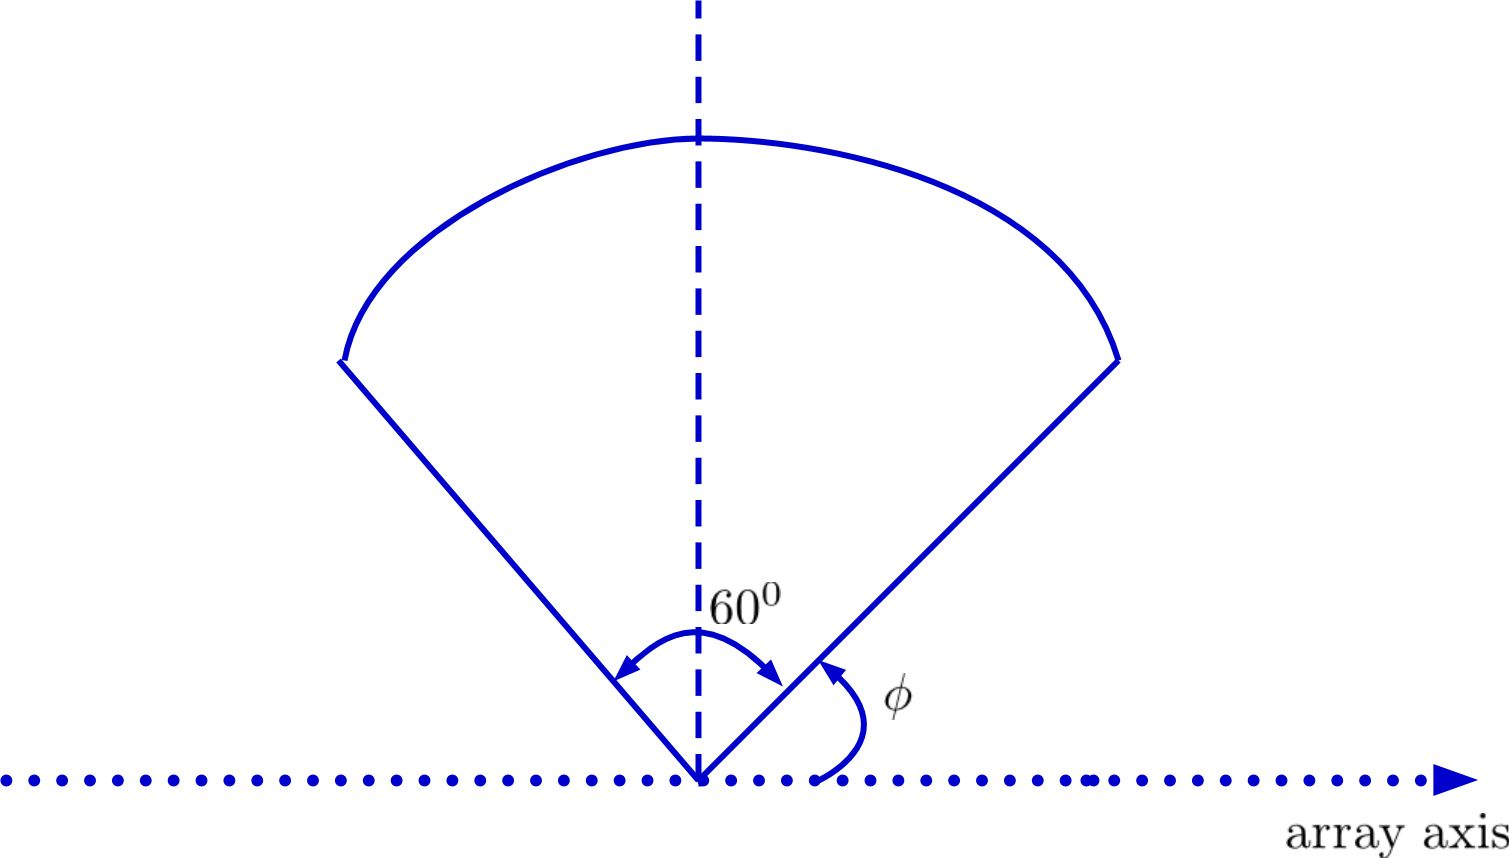
\includegraphics[scale=0.5]{/graphics/img59_4}
% 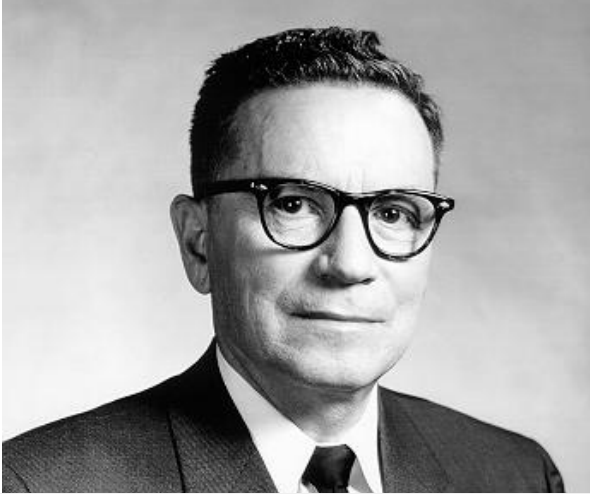
\includegraphics[scale=0.09]{graphics/a21}
\caption{}
\label{fig:fig-3}
\end{figure}

The radiation pattern $f(\phi)$ is given as $\cos(\dfrac{\psi}{2})$ as seen for a 2 element array where $\psi = \beta d\cos\phi + \delta$. Now the radiation pattern of the last two element array of primary pattern $f(\phi)$ is given by the relationship in Equation~\ref{eqn53} as:   $\; f(\phi) \times$ Array factor. \\
Also, the array factor for the last two elements is $\cos(\dfrac{\psi}{2})$.\\
So Radiation pattern = $\cos^2(\dfrac{\psi}{2})$\\
Note that the nulls of the primary radiation pattern are not altered and they correspond to the nulls of the two element array. The Binomial array is important because we can increase the directivity without increasing the nulls in the radiation pattern. It is essential in analysis because for the binomial array of (N + 1) element, we can visualize the array as a combination of two elements (doublets) and essentially each doublet is analyzed to the last two which finally gives the radiation pattern of the array.

\section{General Array Synthesis.}
It is an application where the radiation pattern is specified and then the current excitation can be obtained to realize the arbitrary radiation pattern. This synthesis provides more control of derived properties of the radiation pattern.\\
Let us consider an array of 2N + 1 isotropic elements as shown in fig.\ref{fig:fig-4}. The array distribution is arranged in such a way that there is symmetry of the current distribution about the centre element (reference) in amplitude and phases. Let the current of the $kth$ element be $I_k =a_k + jB_k$ which is a complex quantity and so array phase $\psi =\beta d\cos\phi$ as the phase shift, $\delta$ is contained in $I_k$.
\begin{figure}[h]
\centering
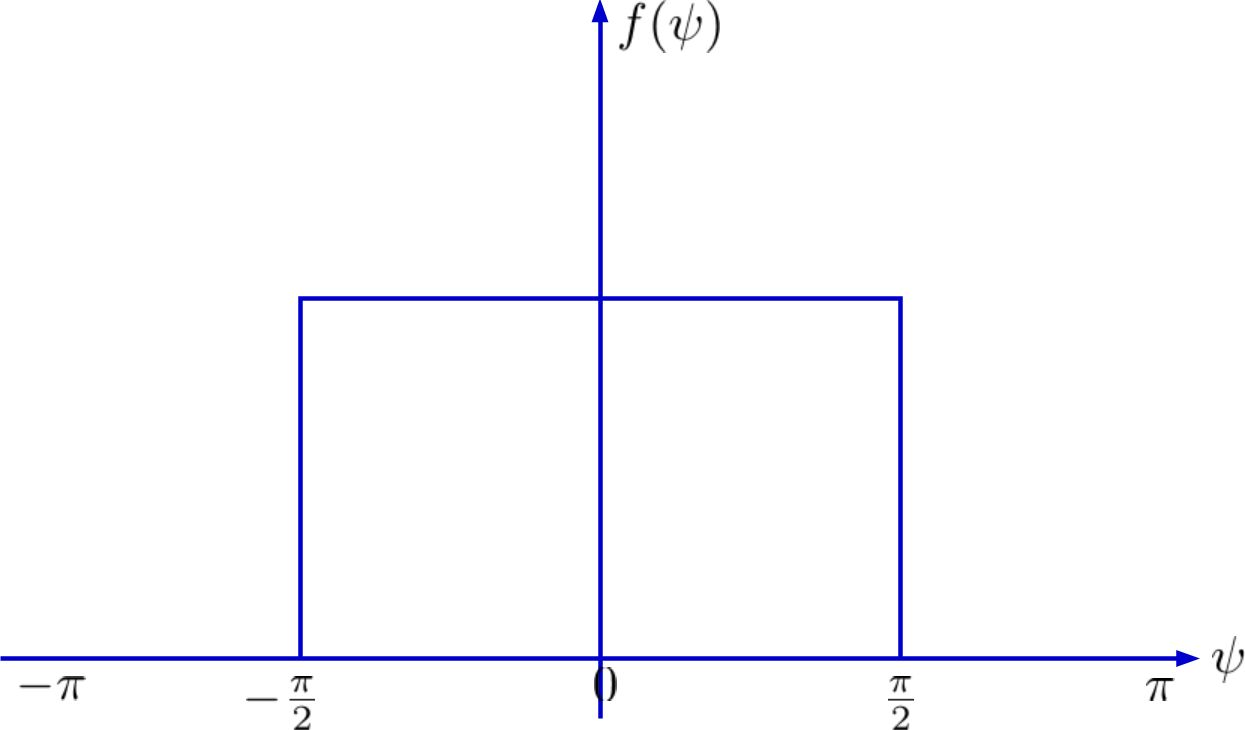
\includegraphics[width=1\linewidth]{/graphics/img59_5}
\caption{}
\label{fig:fig-4}
\end{figure}

The reference current has no phase, so $I_0 = a_0$. The array factor is then given as;\\
$|AF| = |I_0 + I_1 e^{j\psi} + I_2 e^{j2\psi} + \; \cdots \; + I_N e^{jN\psi} + I_1^\ast e^{-j\psi} + I_2^\ast e^{-j2\psi} + \; \cdots|\; + I_N^\ast e^{-jN\psi}$\\
Combining each term with its conjugate,\\
$|AF| = |I_0 + \{I_1 e^{j\psi} + (I_1 e^{j\psi})^\ast\} + \; \cdots \; + \{I_N e^{jN\psi} + (I_N e^{jN\psi})^\ast\}|$\\
$= |I_0 + 2\Re e\{I_1 e^{j\psi}\} + 2\Re e\{I_2 e^{j2\psi}\} + \; \cdots \; + 2\Re e\{I_N e^{jN\psi}\}|$\\
We note the the currents are replaced by $I_k = a_k + jb_k $ and $\Re e\{I_k\ e^{jk\psi}\}$\\
$\Rightarrow \Re e\{(a_k + jb_k)(\cos k\psi + j\sin k\psi)\}$\\
$\Rightarrow a_k\cos k\psi - b_k\sin k\psi$\\
Therefore,
\begin{dmath*}
|AF| = |a_0 + 2(a_1\cos\psi - b_1\sin\psi) + 2(a_2\cos2\psi - b_2\sin 2\psi) + \; \cdots \; + 2(a_N\cos N\psi - b_N\sin N\psi)
\end{dmath*}
\begin{dmath}
|AF| = \left|a_0 + 2\sum_{k=1}^{N} a_k\cos k\psi -2\sum_{k=1}^{N}b_k\sin k\psi\right|
\label{eqn56}
\end{dmath}
which is the fourier series of the array factor and the coefficient which represents the current excitations are the fourier coefficient of the array factor. This relationship has been seen in the fourier transform for a continuous current distribution and it is also seen now for discrete sources. Since the radiation pattern is periodic on $\psi$ then we get its raw fourier transform which is a fourier series. Therefore, if we know the radiation pattern (AF) and if we fourier expand it then the fourier expansion represents the complex current excitation of the elements. It should be emphasized here that for exact representation of a function in general, we need infinite terms in the fourier series. Consequently, the synthesized array factor may be  approximation  to the specified radiation pattern. Larger the number of element in the array, closer is the synthesized pattern to the specified pattern. The array design may therefore be done under two constraints.
\begin{enumerate}[(i)]
\item Acceptible root mean square error between the specified and the synthesized patterns. In this case, there is no control over the number of elements.
\item Pre-decided number of elements. In this case, the fourier analysis gives the best fit (in the least square sense) between synthesized and the specified patterns.
\end{enumerate}
It is also observed that the Fourier synthesis needs the radiation pattern specified in the $\psi$- domain, whereas in practice the pattern is specified as a function of $\phi$. So, we have to convert provided we know $d$ which means prior knowledge of the inter-element spacing $d$ has to be decided by the designer. The visible range of $\psi$ we know is a function of $d$, whereas for the fourier expansion, the period is always $2\pi$. Therefore for a unique synthesis, the inter-element spacing should be equal to $\dfrac{\lambda}{2}$\\
The array synthesis steps are as follows:
\begin{enumerate}
\item[Step 1:] Specify the radiation pattern for $0 \leq \phi \leq \pi$.
\item[Step 2:] Select the inter-element spacing $d$ and the number of elements N in the array (or otherwise specify the rms error between the synthesized pattern and the derived pattern).
\item[Step 3:] Get the radiation pattern as a function of $\psi$. If $d < \dfrac{\lambda}{2},$ there is uncovered range of $\psi$ within $-\pi \; \; \text{and} \; \; \pi$.
\item[Step 4:] Find the fourier series for the function and retain (N + 1) terms including the dc term $(a_0)$.
\item[Step 5:] The excitation currents are the fourier coefficients.
\end{enumerate}
\begin{exmp}
Design an array of five (5) elements whose array factors is given as\\
$ AF = \begin{cases}
1 \; \; \; \; \dfrac{\pi}{3} \leq \phi \leq \dfrac{2\pi}{3}\\
\\
0 \; \; \; \; \text{otherwise}
\end{cases}$.
Determine the excitation of the antenna elements which will produce this radiation pattern. Choose $d = \dfrac{\lambda}{2}.$
\begin{figure}[h]
\centering
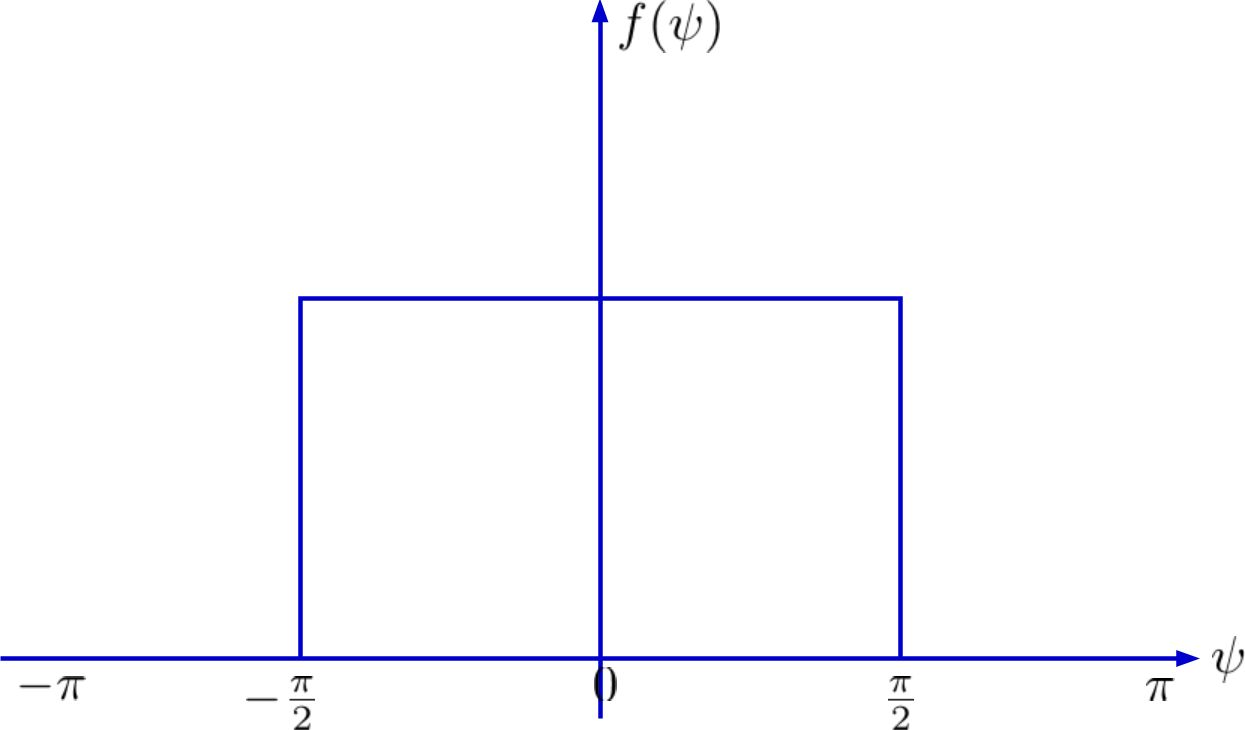
\includegraphics[width=1\linewidth]{/graphics/img59_5}
\label{fig:fig-5}
\end{figure}

\subsection{\centering Solution}
Given: $\psi = \beta d \cos\phi = \dfrac{2\pi}{\lambda} \cdot \dfrac{\lambda}{2} \cos\phi = \pi\cos\phi$\\
\\
So, $AF = f(\psi) =\begin{cases}
1 \; \; \; \; \dfrac{\pi}{3} \leq \phi \leq \dfrac{2\pi}{3}\\
\\
0 \; \; \; \; \text{otherwise}
\end{cases}$. 
\begin{figure}[h]
\centering
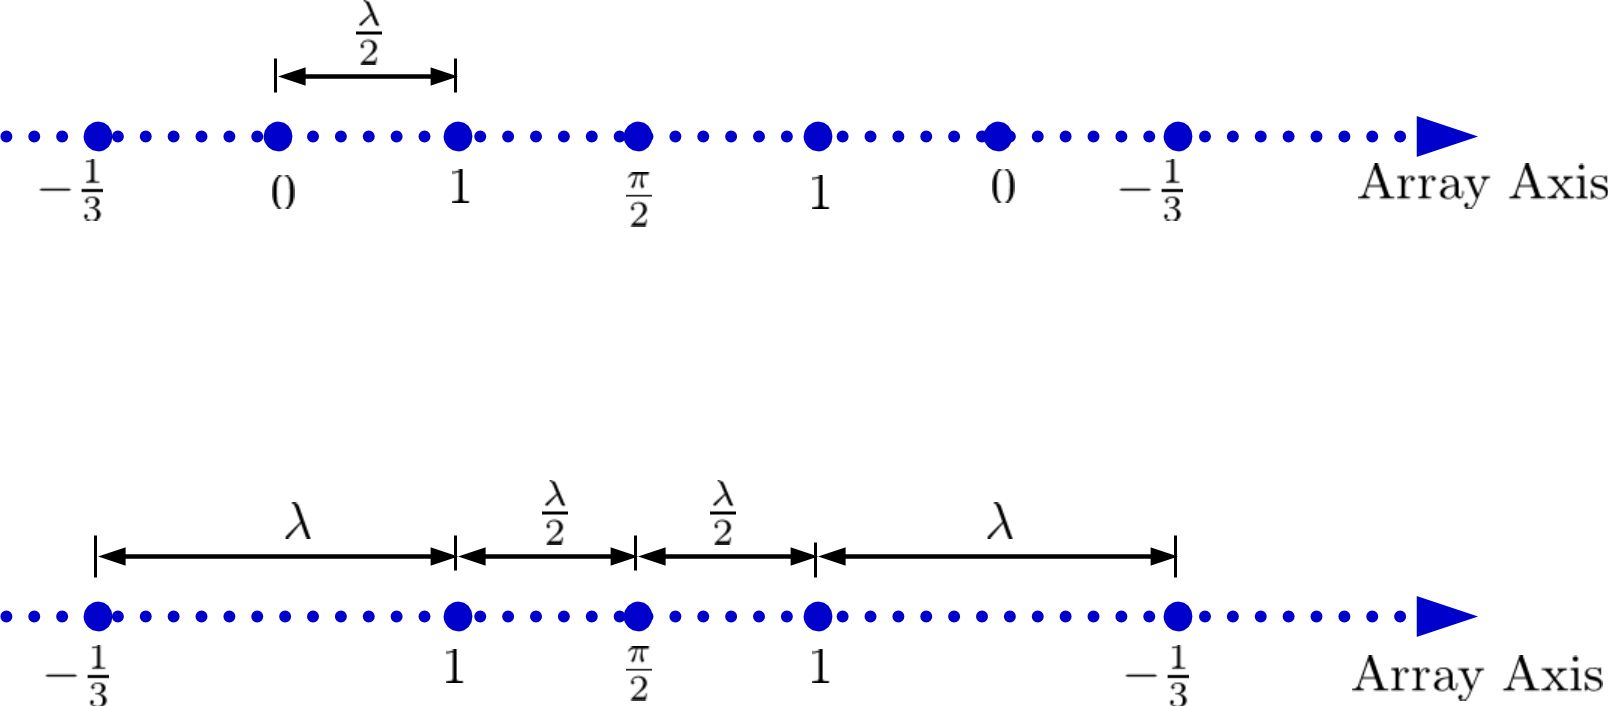
\includegraphics[width=1\linewidth]{/graphics/img59_6}
\label{fig:fig-6}
\end{figure}

Fourier series of $AF =
a_0 + 2 \sum_{k = 1}^{2}a_k\cos k\psi - 2 \sum_{k = 1}^{2}b_k\sin k\psi
\label{sum}
$

We have that the coefficients are given as follows over a period of $2\pi$
$$a_0 = \dfrac{1}{2\pi}\int_{-\pi}^{\pi}|AF|d\psi = \dfrac{1}{2\pi}\int_{-\dfrac{\pi}{2}}^{\dfrac{\pi}{2}}d\psi = \frac{1}{2}$$
Also;
$$a_k = \dfrac{1}{2\pi}\int_{-\pi}^{\pi}|AF|\cos k\psi d\psi = \dfrac{1}{2\pi}\int_{-\dfrac{\pi}{2}}^{\dfrac{\pi}{2}}\cos k\psi d\psi$$
$$= \dfrac{1}{k\pi}\sin(\dfrac{k\pi}{2})$$ and $b_k = 0$\\
Therefore, we have\\
$ a_0 = \dfrac{1}{2}, \; \; a_1 = \dfrac{1}{\pi},\; \; a_2 = 0, \; \; a_3 = -\dfrac{1}{3\pi}, \; \;a_4 = 0$.\\
The array factor from Equation~\ref{eqn49} is given as:\\
$-\dfrac{1}{3\pi}z^{-3} + 0 +\dfrac{1}{\pi}z^{-1} + \dfrac{1}{2} + \dfrac{1}{\pi}z + 0 - \dfrac{1}{3\pi}z^{3}$\\
$= \dfrac{1}{\pi}\{
-\dfrac{z^{-3}}{3} + z^{-1} + \dfrac{\pi}{2} + z - \dfrac{z^3}{3}
\}$\\
NOTE: Since $a_2 = 0$, we have included $a_3$ in the expansion (for five element array). If $a_2$ were not equal to zero, $a_0, \; a_1, \; a_2 \;$ would have made five elements in the array. The array element spacing and current excitation of the designed array as shown in fig \ref{fig:fig-7} below.
\begin{figure}[h]
\centering
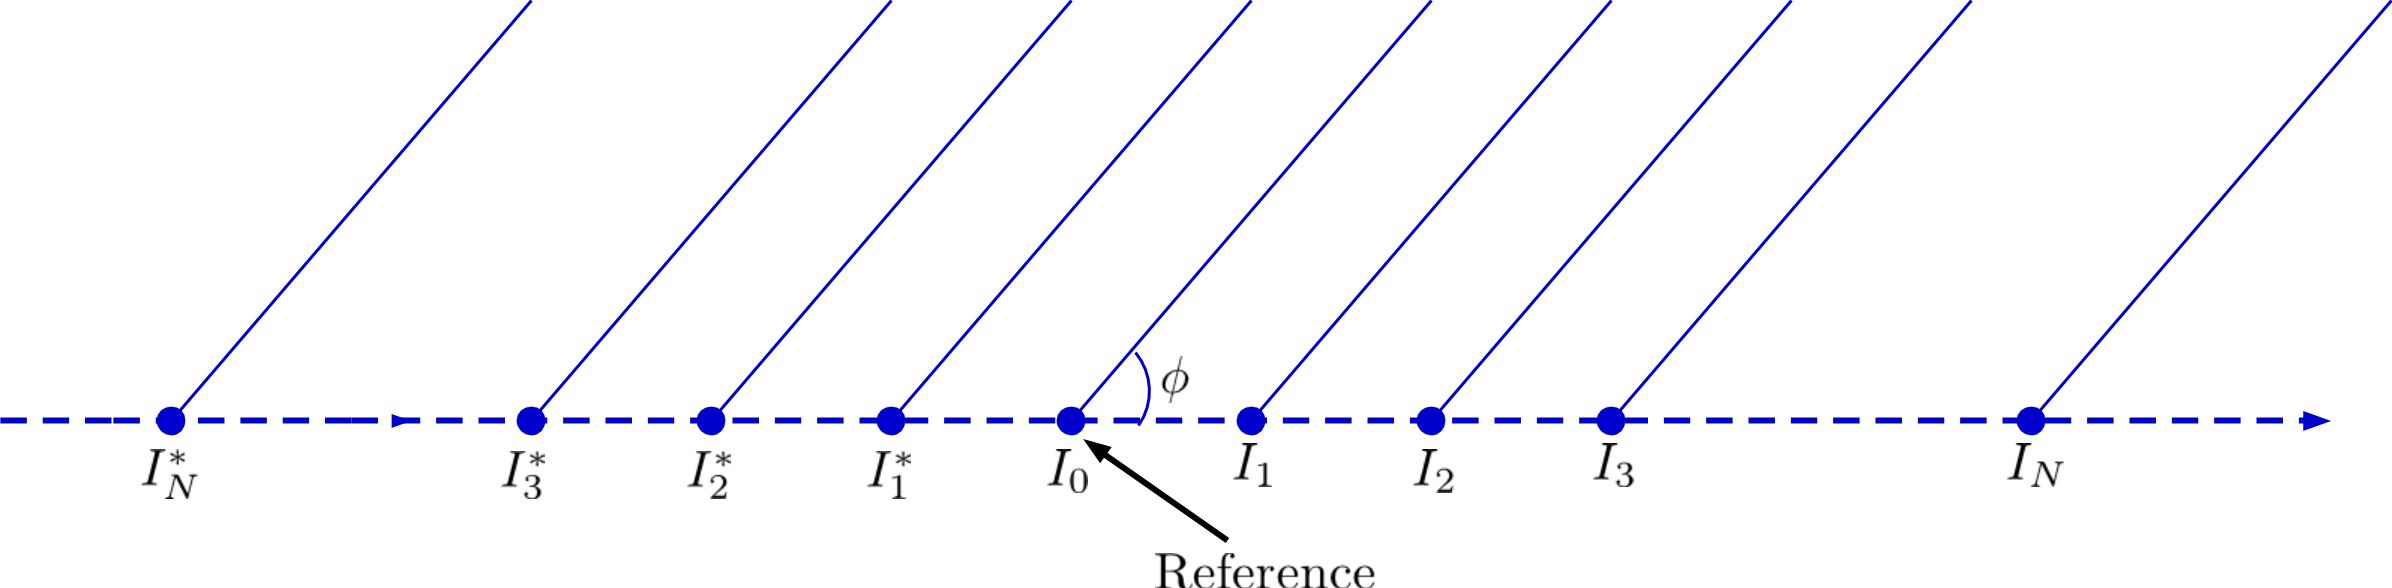
\includegraphics[width=1\linewidth]{/graphics/img59_8}
\caption{}
\label{fig:fig-7}
\end{figure}

\end{exmp}
\begin{ExerciseList}
\Exercise[title=DIY]
\Question{Design an end-fire array to have sectoral beam only in one direction along the axis of the array (take $d = \dfrac{\lambda}{4}$). The maximum number of elements permitted is seven and the width of the beam is $90^0$\\
\begin{figure}[H]
\centering
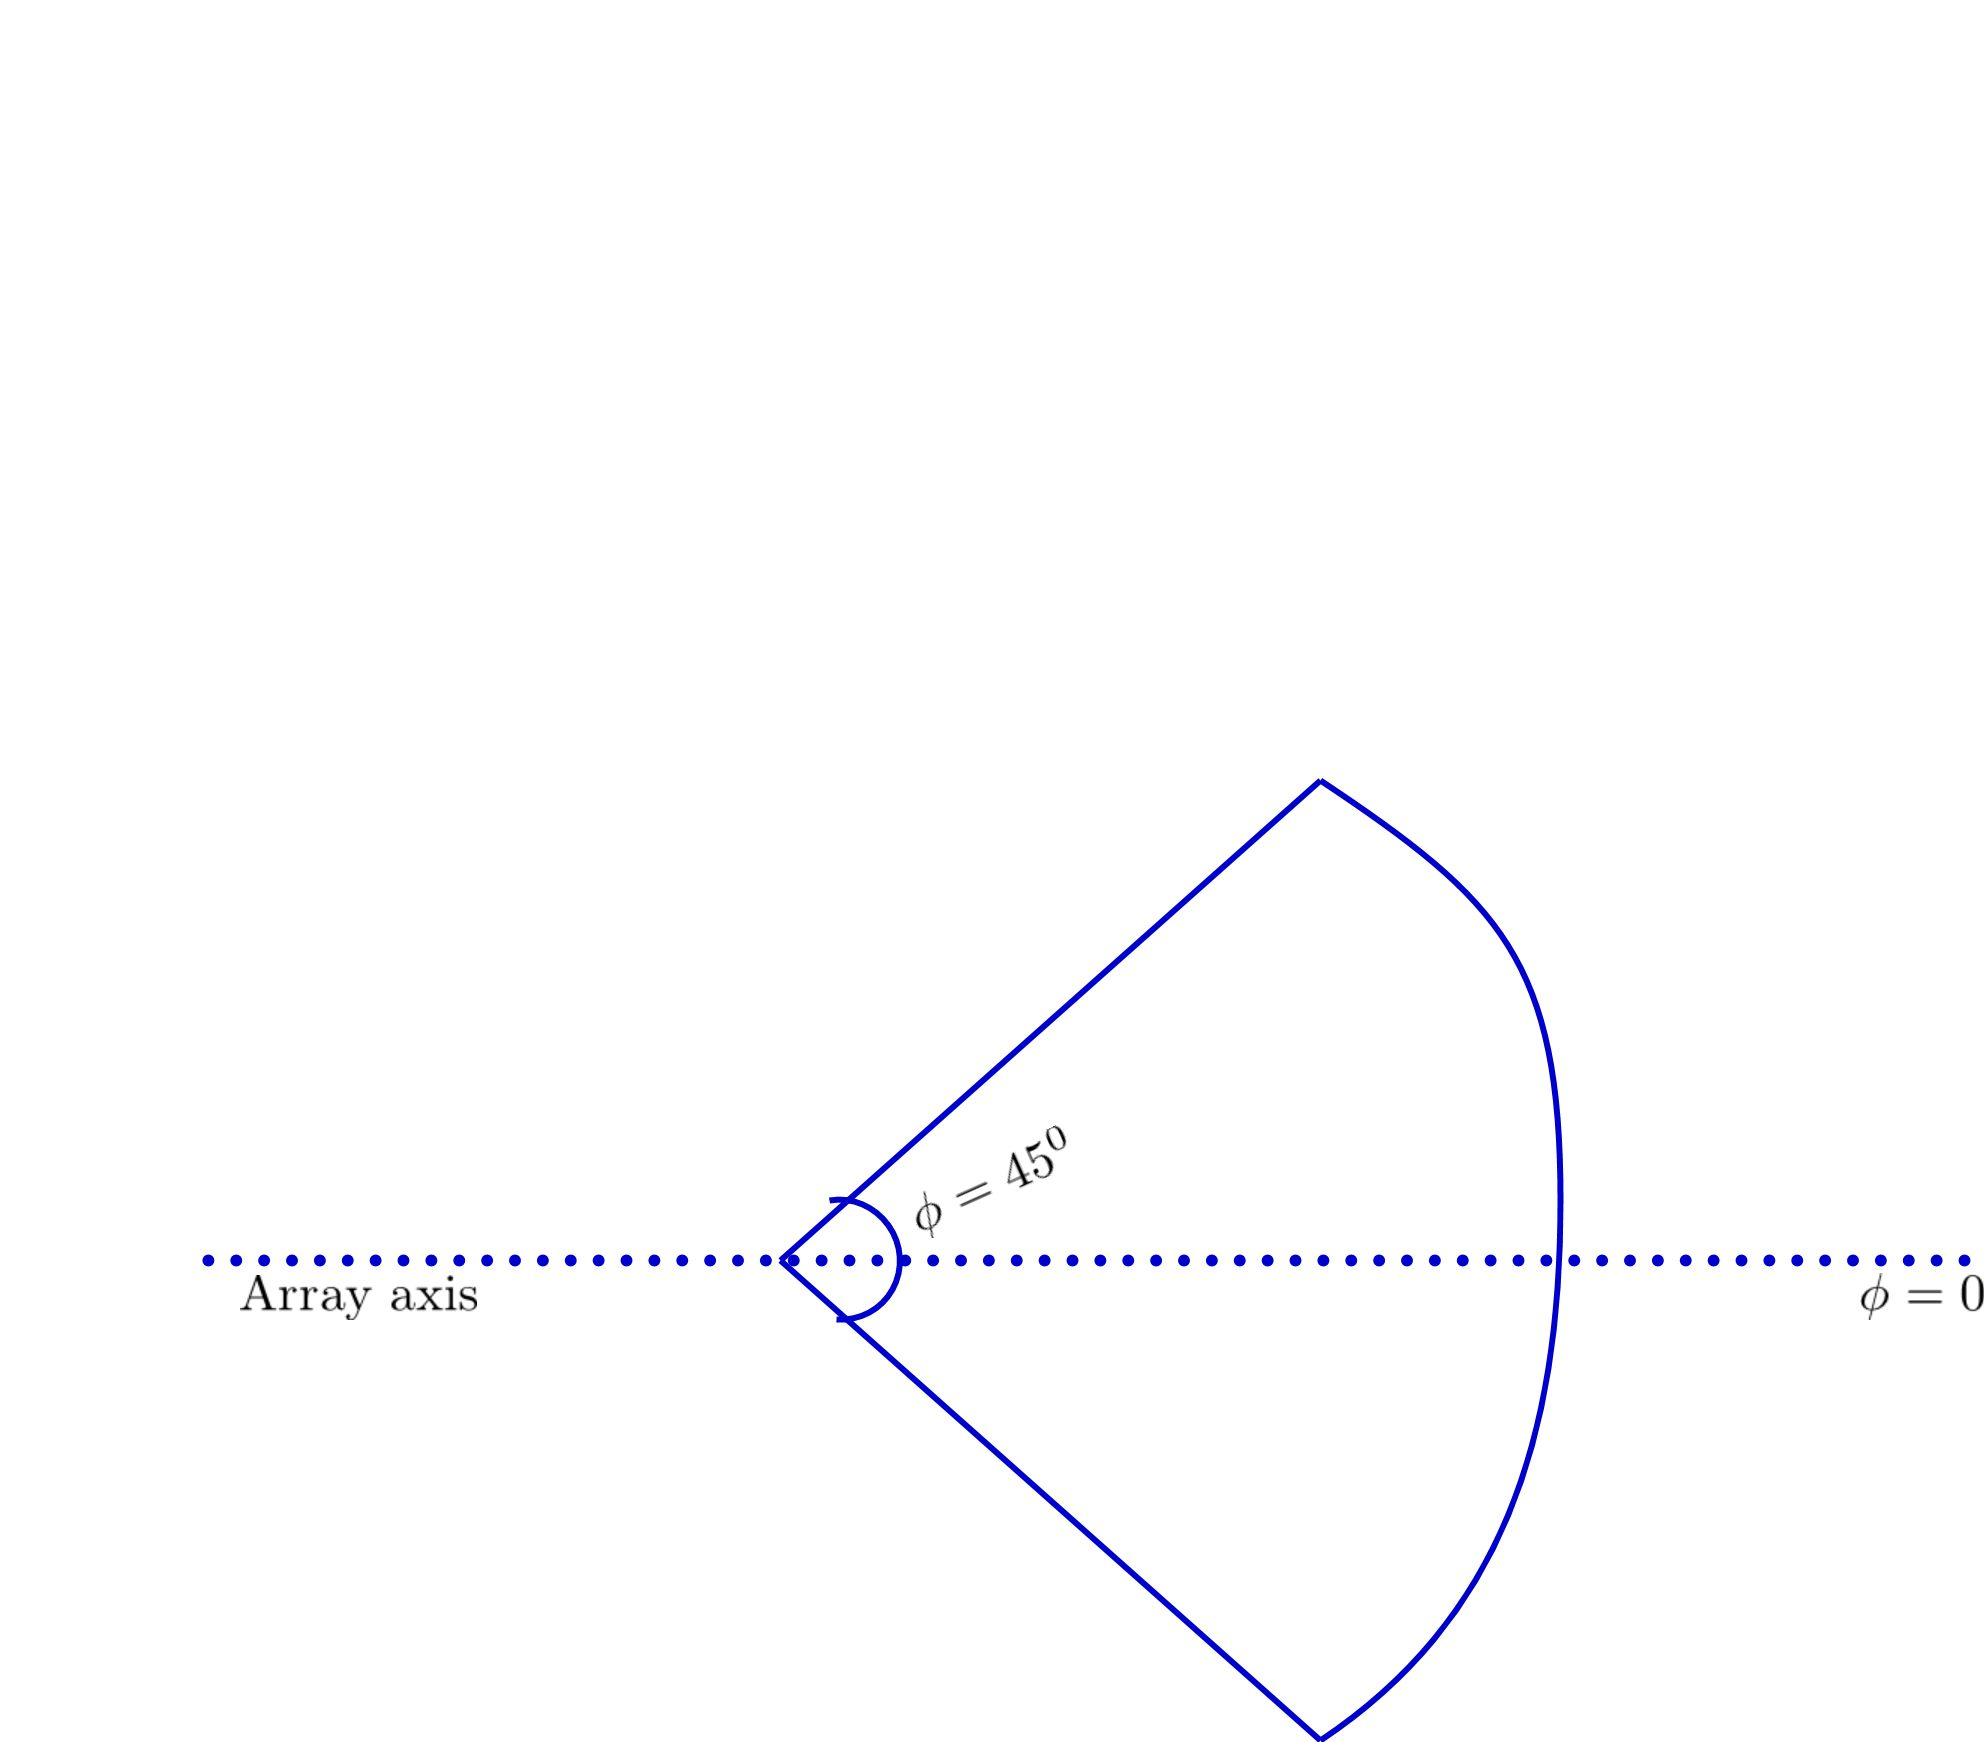
\includegraphics[width=1\linewidth]{/graphics/img59_7}
\caption{Desired radiation pattern}
\label{fig:fig-8}
\end{figure}}
\end{ExerciseList}

Essentially, this completes the discussion on array synthesis.